\chapter{Background Material: on Convolutional Neural Networks}

\noindent We start with a brief review of feedforward neural networks before elaborating on convolutional neural networks (CNNs). A number of good books available expand on the following content in much greater detail, notably \citep{Bengio-et-al-2015-Book}, \citep{Bishop:1995:NNP:525960} and \citep{Nielsen}.

\section{Feed Forward Neural Networks}

\begin{figure}
\centering
%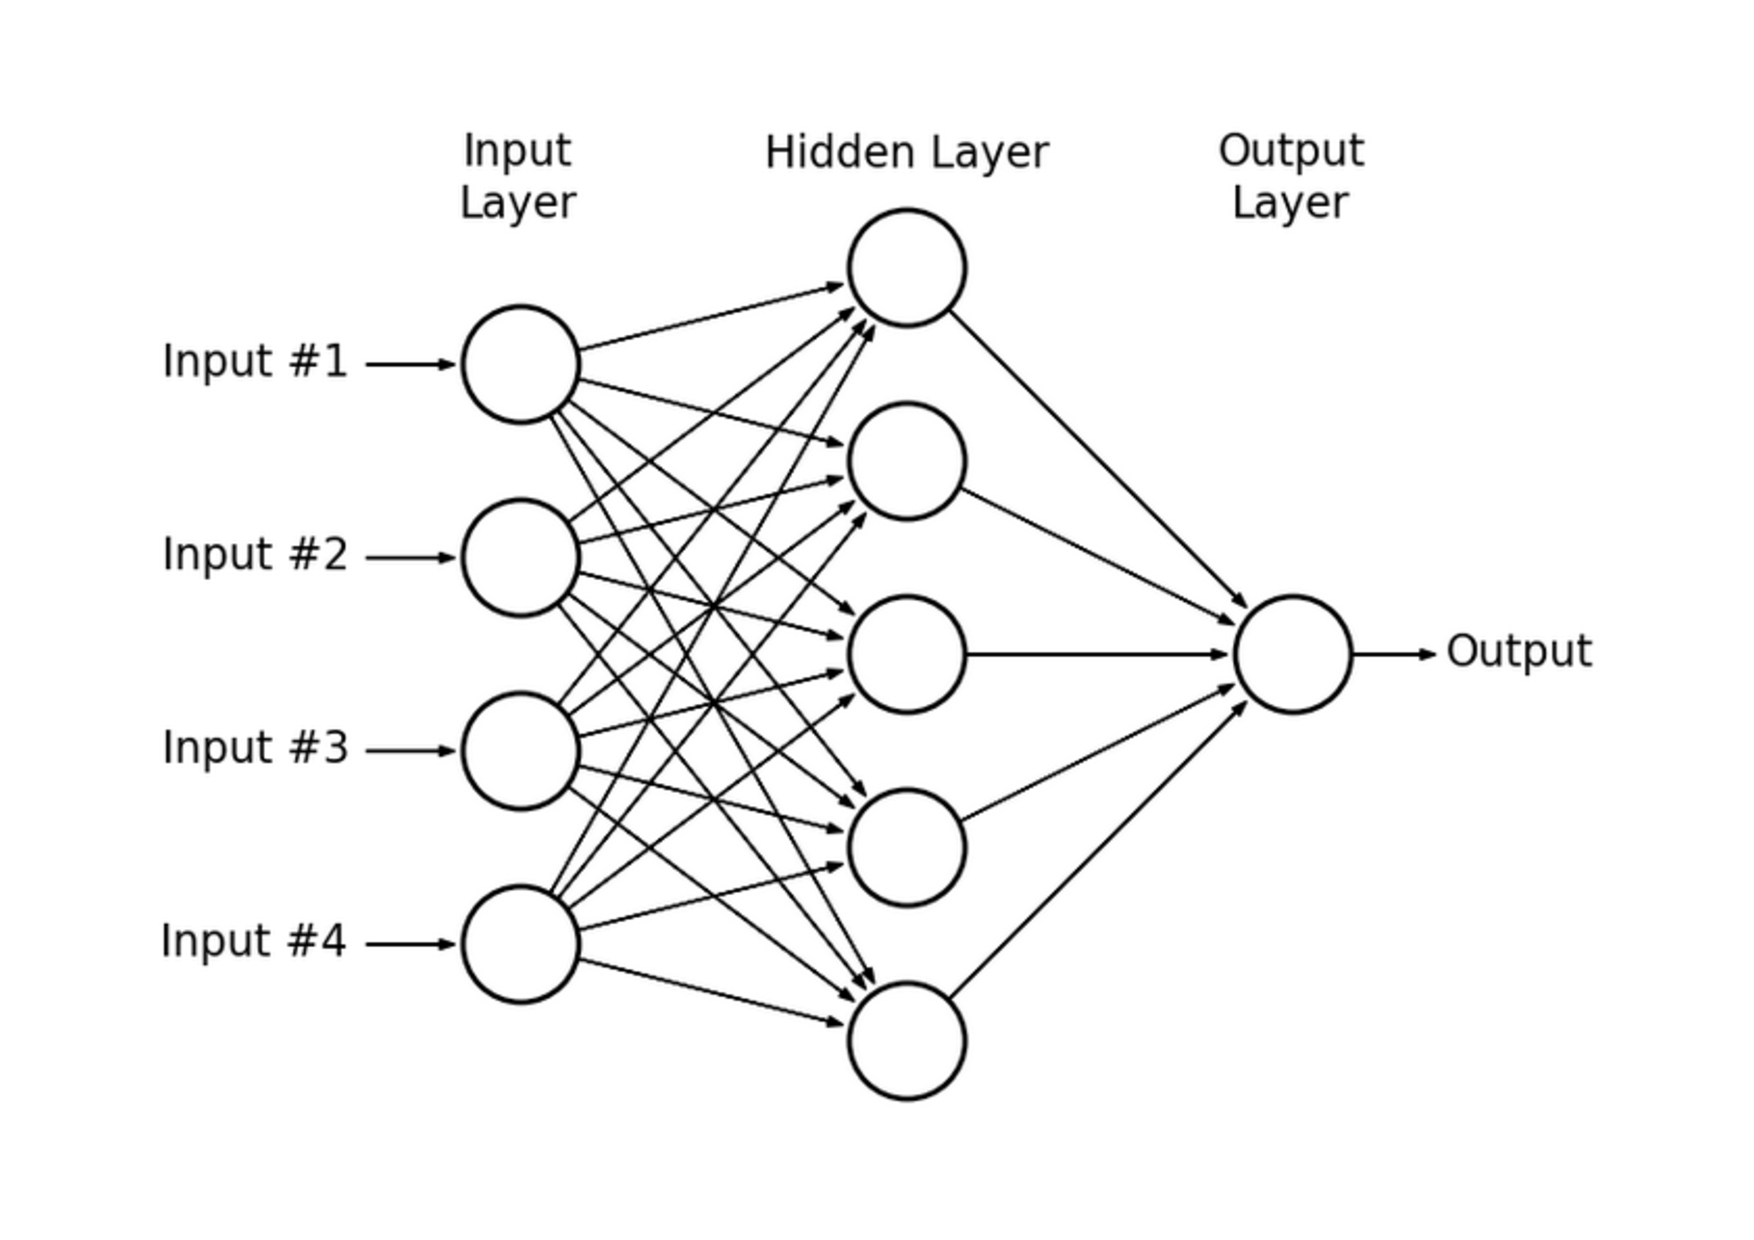
\includegraphics[trim=2cm 2cm 2cm 2cm, clip=true, height=80mm]{Chapter2/FF_Neural_Network.pdf}
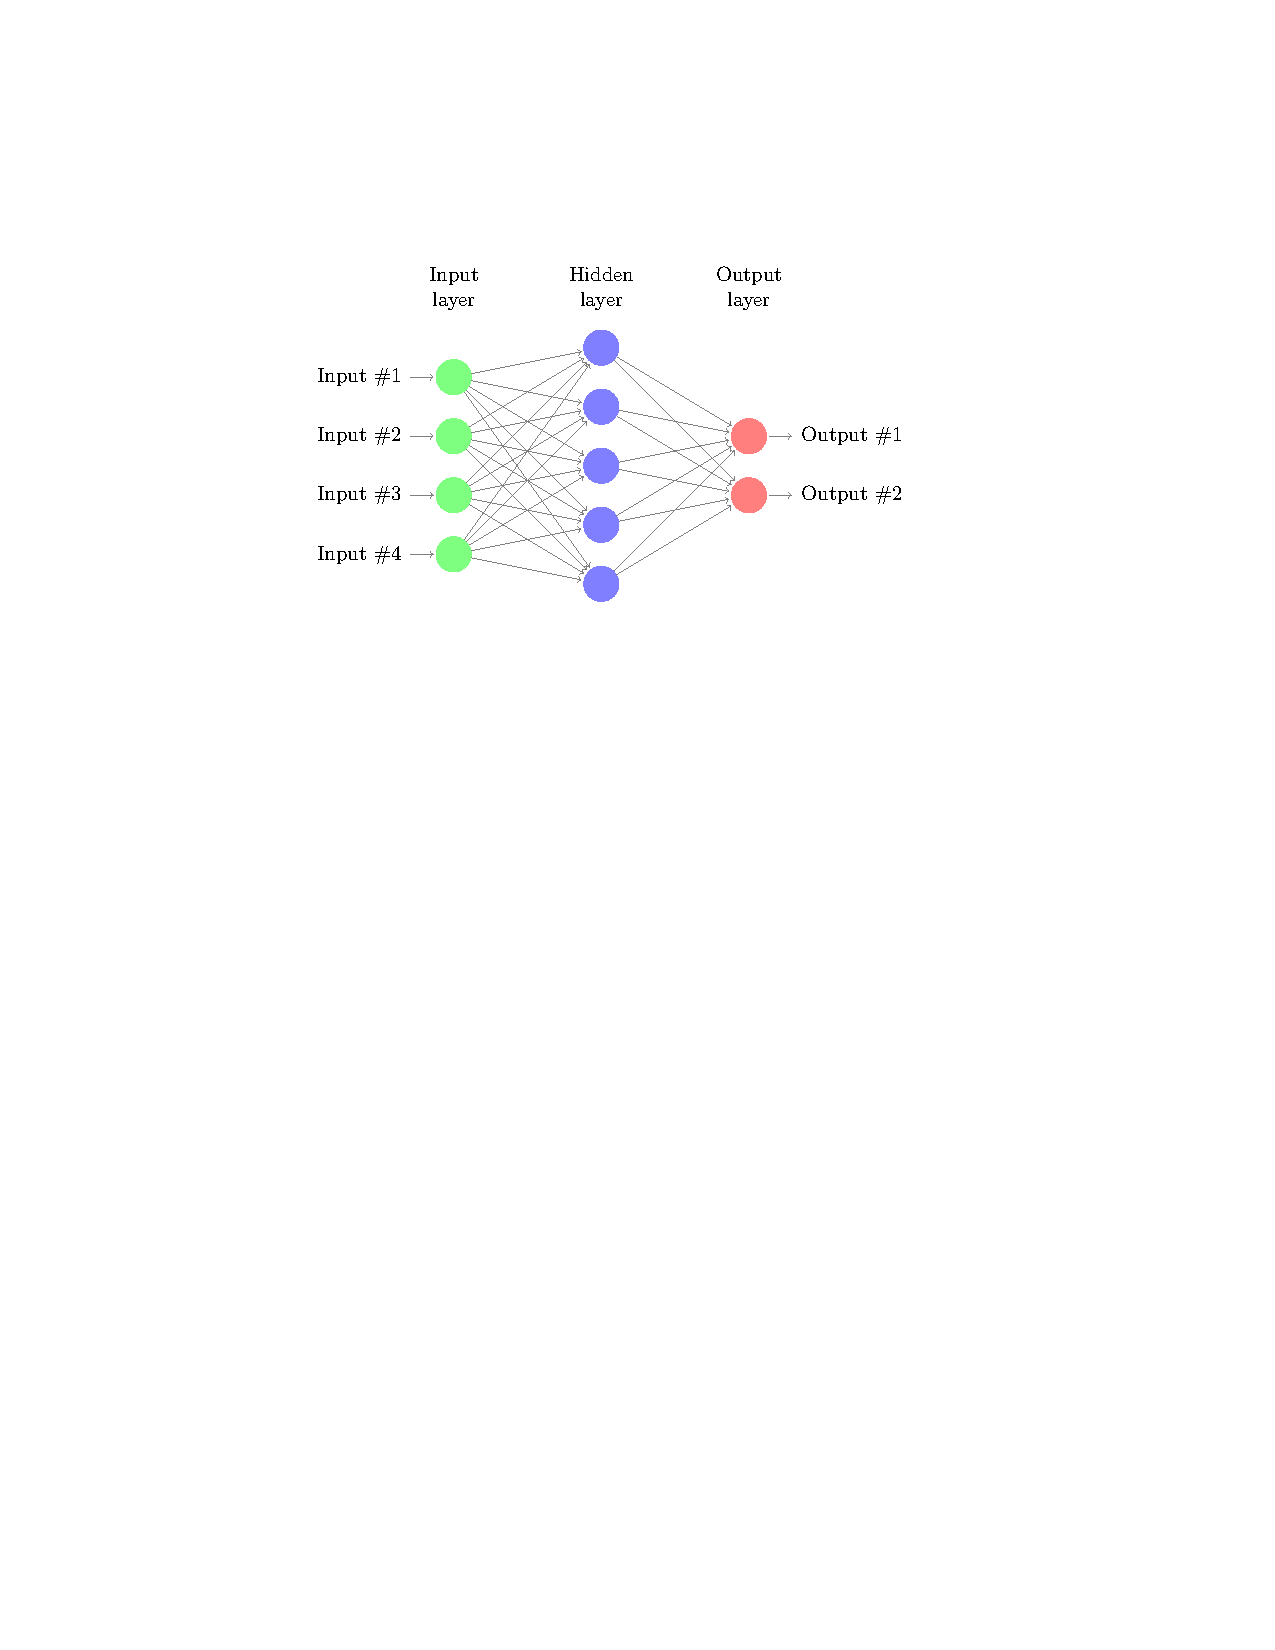
\includegraphics[trim=4cm 17cm 3cm 4cm, clip=true, height=80mm]{Tikz/NN.pdf}
\caption{A 1 layer-feedforward neural network with 4 input nodes, 1 hidden layer with 5 hidden nodes and 2 output node.}
\label{Basic_neural_network}
\end{figure}

A feedforward neural network is a standard model in the machine literature for classification problems. It consists of a number of layers composed of simple processing units, also called neurons or nodes, in which each unit in a given layer is connected to a number of units in the previous layers, each connection characterised by a weight encoding the knowledge of the network. Layers in which every unit is only connected to every unit in the previous layer are called fully-connected layers. Each unit represents an activation value generated by passing a linear combination of the values of the incoming connections weighted by their weights to an activation function, such as a Rectified Linear, a Tanh or a Sigmoid function. The information encoded in the data enters at the input layer, gets processed as it passes through the network, layer by layer, until it arrives at the output layer. The choice of the activation function at the output layer is determined by the nature of the data and the assumed distribution of the target variables. For classification problems, the softmax function or, in our case, its log, give the output a probabilistic interpretation. This model can be represented in the form of a network diagram as shown in Figure \ref{Basic_neural_network}.\\

\noindent Training a neural network is done by minimising an error measure of its performance over a training set using gradient-based optimisation routines. The error gradients with respect to the parameters that are needed for the minimisation procedure, can be efficiently evaluated via the standard backpropagation algorithm. To prevent overfitting, a number of regularisation methods are available, including the traditional ones such as L1 and L2 regularisation. Recently a method called dropout \citep{JMLR:v15:srivastava14a} where at every epoch, a percentage of hidden units are randomly deactivated during training has been shown to give better generalisation performance.

\section{Convolutional Neural Networks}

\noindent A CNN is a specialised kind of feedforward neural network where the first few layers of the architecture are so-called convolutional layers. These consist of three stages: a convolution stage, a detection stage and an optional subsampling stage. We will be discussing CNNs in the context of multi-channel images of size $m \times m$, where each pixel value represents an input node. 

\subsection{Convolution}

\begin{figure}
\centering
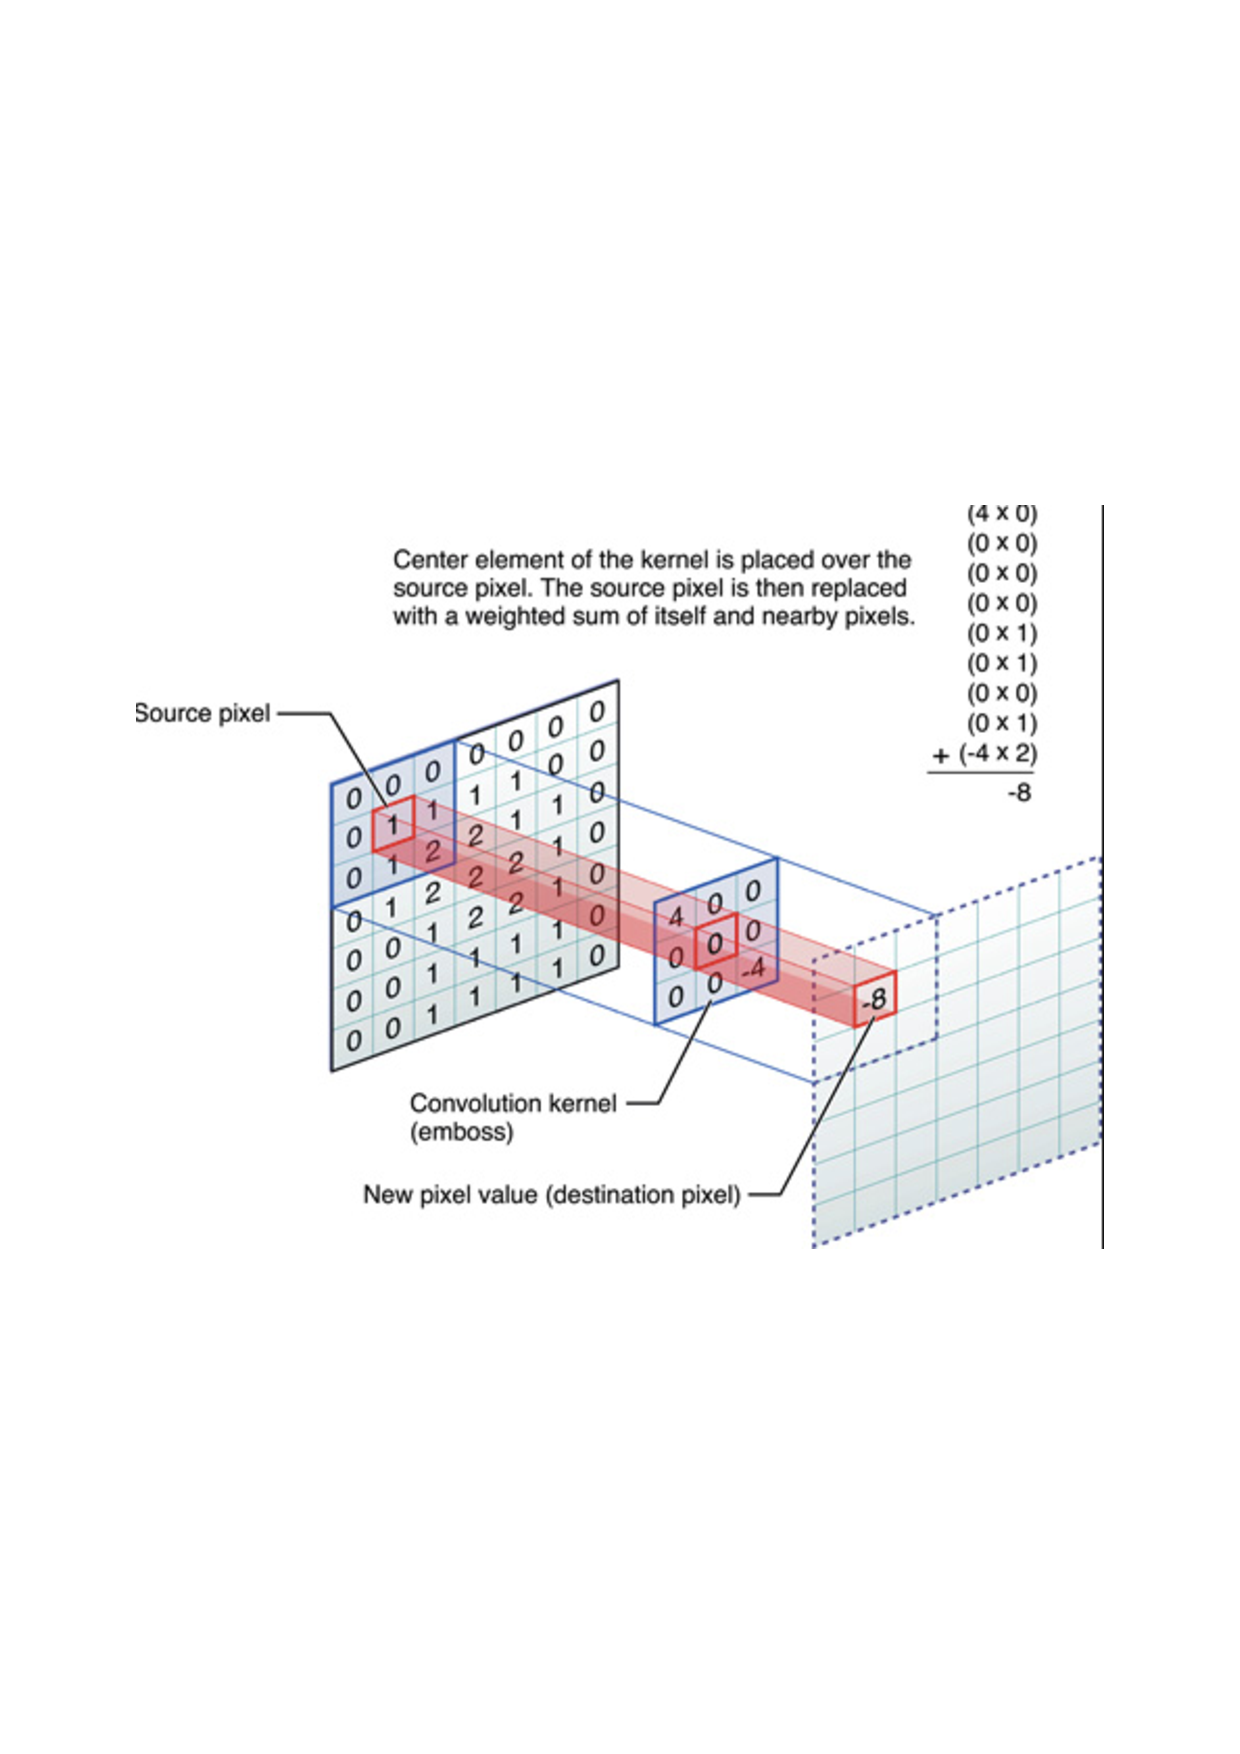
\includegraphics[trim=2cm 7cm 2cm 7cm, clip=true, height=80mm]{Chapter2/convolution.pdf}
\caption{The convolution layer. Illustration of the formation of a feature map taken from \citep{url_convolution}}
\label{convolution_operation}
\end{figure}

\noindent The convolution stage is responsible for implementing $k$ convolution operations over each channel of the input image. This is accomplished by convolving in parallel each channel with $k$ kernels of size $s \times s$. Unlike fully connected layers, in a convolution, each output node is locally connected to a small square subset of corresponding input nodes determined by the kernel size. Additionally, as the same kernel is applied throughout the image, the convolution operation implies weight sharing, thus greatly reducing the number of trainable parameters. Figure \ref{convolution_operation} illustrates the convolution operation graphically. The set of output nodes resulting from one kernel is called a feature map, which is itself a rectangular arrays of nodes of size $(m - s/2 + 1) \times (m - s/2 + 1)$. Feature maps detect the presence in the input image of a particular feature encoded by the corresponding kernel. Having multiple kernels run through the input layer in parallel produces a set of feature maps. Together, they are responsible for detecting various types of features which might be present in the image. \\

\noindent The benefits of this approach are two folds :

\begin{itemize}
	\item Computational efficiency: the sparse interaction between the hidden nodes and the weight sharing significantly decrease the number of parameters to train.
	\item Translational equivariance: shifting the input results in an equivalent shift in the output. This is a property of the convolution operation.
\end{itemize}

\noindent In the detector stage, every node in the feature map is then passed to an nonlinear activation unit exactly as in a standard neural network. These activation units usually consist of either Rectified Linear units (ReLU), Tanh units, or Sigmoid units.\\

\begin{figure}
\centering
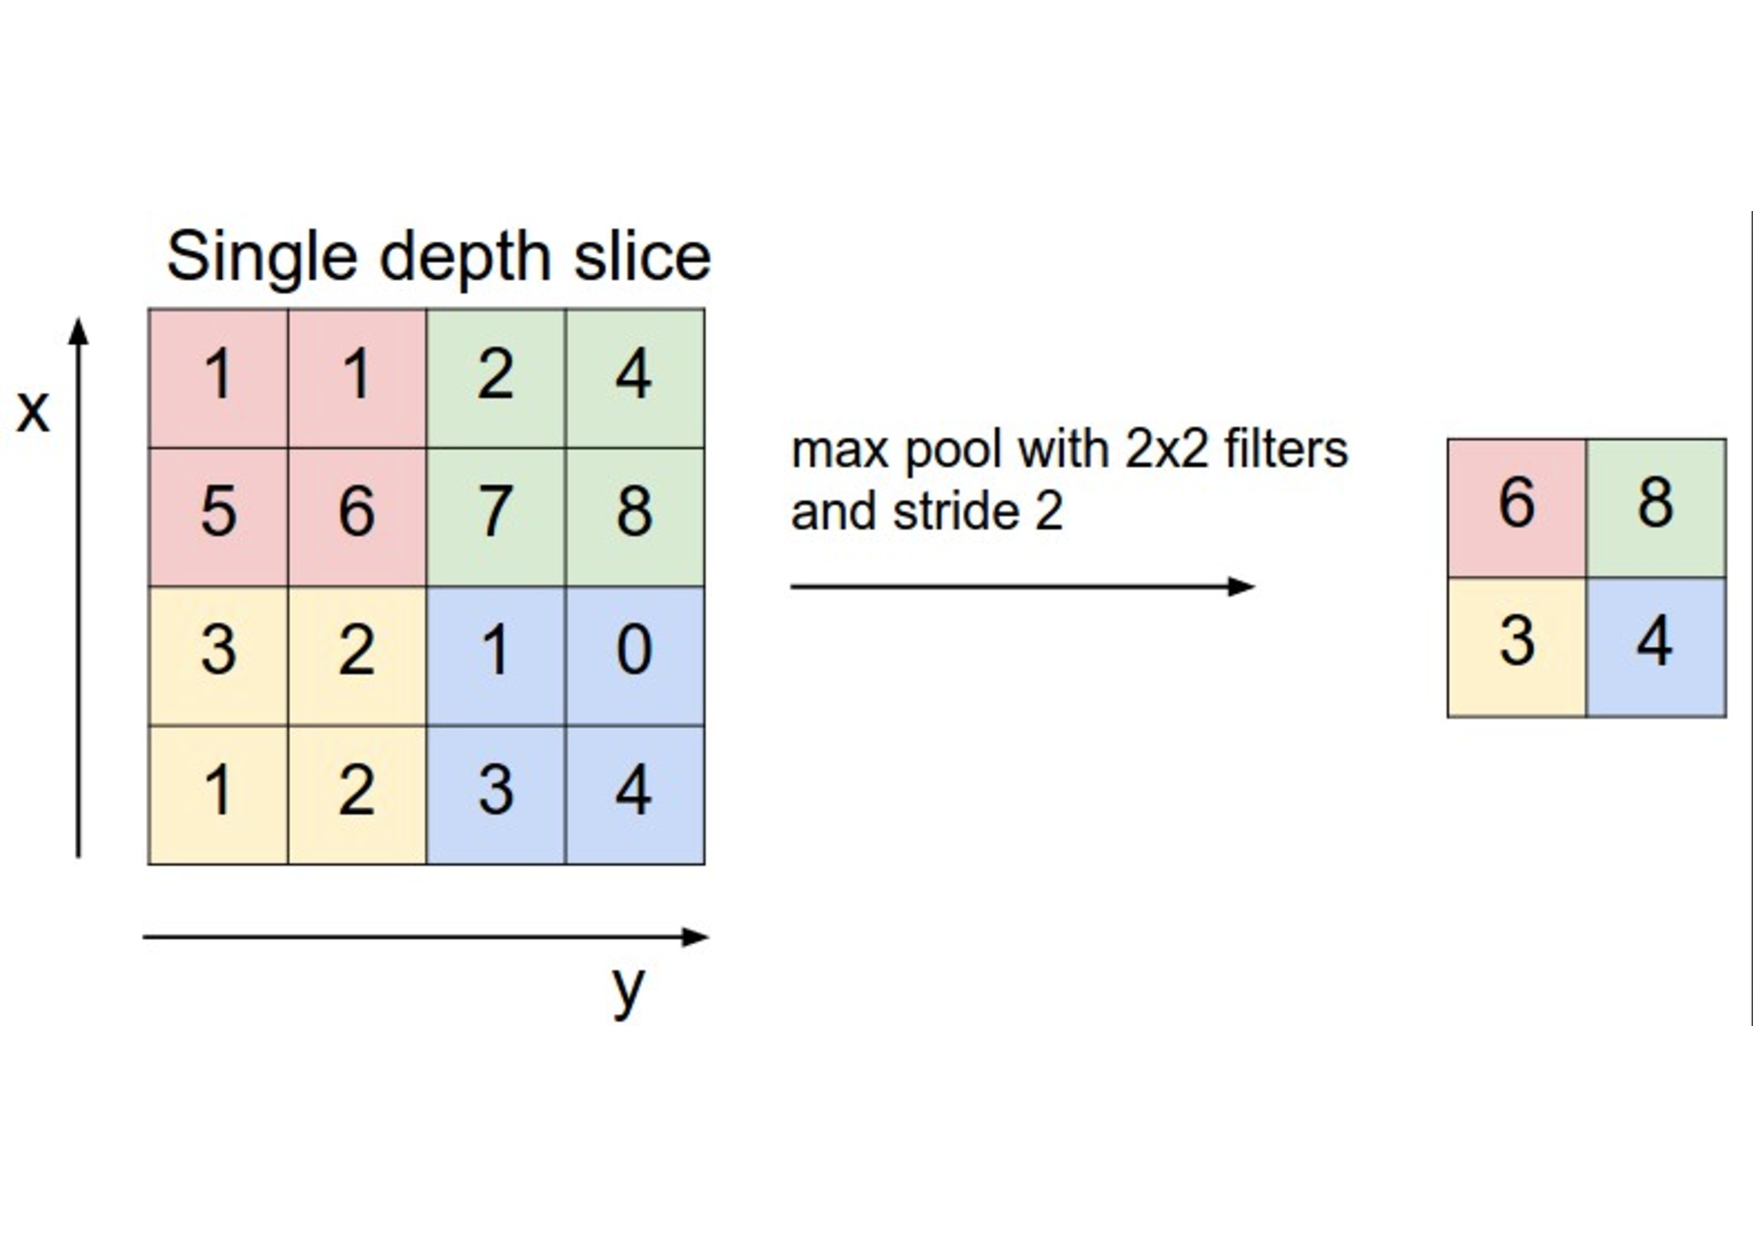
\includegraphics[trim=0cm 0cm 0cm 0cm, clip=true, height=60mm]{Chapter2/pooling.pdf}
\caption{Subsampling in action. Here maxpooling is used to halve the size of an feature map using a $2 \times 2$ filter}
\label{subsampling}
\end{figure}

\noindent Finally in the pooling stage, each feature map is then subsampled by aggregating the node values using a summary statistic over a rectangular neighbourhood of outputs. Two commonly used ones are the max and average pooling operations which report respectively the maximum and average of a set of inputs. Figure \ref{subsampling} shows a diagram of subsampling.\\

\noindent The benefits of subsampling are that it further reduces the number of features by a factor of k for pooling regions spaced k pixels apart, aiding the classification task and improving the computational efficiency of the network. Furthermore subsampling has the added benefit of making the representation become invariant to small translations of the input. Thus translating the input by a small amount results in little to no change in the values of the pooled outputs.\\

\subsection{Typical Architecture}

\noindent A typical convolutional neural network architecture consists of an input layer, a number of convolutional layers, a number of fully connected layers, followed by an output layer. The input layer is an $r \times n \times n$ image, with $r$ being the number of channels and $n$ the image height and width. Each channel is passed through a number of convolutional layers in parallel. Then the remaining output nodes from all the resulting feature maps across all channels are "flattened" and passed as input to a number of fully connected layers. The output layer classifies the input into one of a number of different classes. The convolutional layers thus serve as a way to reduce the dimensionality of the image by extracting meaningful local features.







